\documentclass[12pt]{article}
\usepackage{geometry}
\usepackage{titlesec}
\usepackage{enumitem}
\usepackage{hyperref}
\usepackage{graphicx}
\usepackage{todonotes}
\usepackage{float}
\usepackage{amsmath}
\usepackage{tikz}
\usetikzlibrary{positioning, shapes.geometric, arrows.meta}

\geometry{a4paper, margin=1in}
\titleformat{\section}{\large\bfseries}{\thesection}{1em}{}
\titleformat{\subsection}{\normalsize\bfseries}{\thesubsection}{1em}{}

%-------------Ttitle Page-------------
\begin{document}

\begin{titlepage}
    \centering
    \vspace*{\fill}

    {\LARGE \textbf{Final Year Project: Preliminary Report}}\\[2em]
    {\large Development of an Explainable Deep Learning Model for}\\[0.5em]
    {\large Early Breast Cancer Detection in Singaporean Women with Dense Tissue}\\[4em]

    {\large \textbf{Justin Lim}}\\[1em]
    {\large \today}

    \vspace*{\fill}
\end{titlepage}
\newpage
\tableofcontents
\newpage

%-------------Introduction Page-------------
\newpage
\section{Introduction}

\subsection{Project Template}
3.2 Project Idea 2: Deep Learning Breast Cancer Detection 

\subsection{Project Background Information}
Breast cancer remains the most common cancer among women in Singapore~\cite{10}. While national screening programs such as BreastScreen Singapore aim to improve early detection, multiple barriers—such as dense breast tissue, lower participation among certain ethnic groups, and limitations in clinical capacity—still affect screening efficacy. As shown in the Singapore Breast Cancer Cohort (SGBCC) and recent public health literature, under-screening and delayed diagnosis are especially prominent among older women and specific demographic groups. 

This project addresses these challenges by developing a localized, explainable AI system that enhances early detection for high-risk cases. The value lies in improving diagnostic accuracy in dense breast tissue scenarios, increasing clinician trust through explainability, and supporting targeted interventions in under-screened populations.

\subsection{Project Concept}
This project proposes an explainable deep learning system that classifies histopathology or mammography images to support breast cancer detection. The system is optimized for diagnostic workflows in Singapore, particularly for patients with dense breast tissue or late-stage presentation. Convolutional Neural Networks (CNNs), combined with interpretability tools such as Grad-CAM, will be used to generate heatmaps that highlight model attention areas, allowing clinicians to visually validate predictions.

\subsection{Project Objectives}
The main objectives of this project are:
\begin{itemize}
    \item To design and train a CNN-based model that accurately classifies breast cancer from mammography or histopathology image datasets.
    \item To evaluate model generalization performance on profiles relevant to Singaporean women, particularly those with dense breast tissue and older age.
    \item To integrate explainability features such as Grad-CAM that generate visual outputs aligned with known diagnostic markers, thereby increasing clinician trust and interpretability.
\end{itemize}

\subsection{Deliverables}
\begin{itemize}
    \item A trained and tested CNN-based image classification model (e.g., ResNet or EfficientNet)
    \item Grad-CAM visualizations for model interpretability
    \item Evaluation metrics (e.g., accuracy, sensitivity, specificity, F1-score) measured across typical and edge-case scenarios
\end{itemize}


\newpage

%-------------Literature Review Page-------------
\newpage
\section{Literature Review}

This chapter reviews the limitations of traditional breast cancer risk models, the role of deep learning in diagnostic imaging, the importance of explainability, and challenges in generalizing models across diverse populations. Each section provides justification for the design choices and objectives outlined in this project—emphasizing the need for a localized, explainable deep learning system in Singapore's screening context.

\subsection{Limitations of Traditional Risk Models}

Risk prediction models form the foundation of clinical decision-making in early breast cancer detection. Conventional tools, such as the Gail and Tyrer-Cuzick models~\cite{1}, have been widely adopted in clinical settings for population-level risk stratification. These models use structured demographic and clinical inputs to estimate cancer risk but are limited by their rule-based design and assumptions of feature independence.

For this project, understanding the limitations of these traditional models is crucial—they underscore the need for more individualized and image-informed approaches. These models are unable to capture spatial or visual features present in medical images, which are essential when diagnosing cancer in women with dense breast tissue.

A key study~\cite{1} compared the Tyrer-Cuzick model with CNN-based deep learning models trained directly on mammograms. The deep learning models significantly outperformed the clinical models, with AUC values ranging from 0.68 to 0.70 compared to 0.62. These results were especially compelling for dense breast tissue subgroups—directly aligning with this project’s target population of Singaporean women, who often present with dense tissue at younger ages~\cite{6}.

Appendix Figure~\ref{fig:lit1table2} further illustrates these findings. It shows that the deep learning model identified over 31.2\% of future cancers within the highest-risk decile—almost double the detection rate of the Tyrer-Cuzick model, which captured only 18.2\%. This performance gap highlights not just improved sensitivity, but also the model’s utility in stratifying high-risk cases early—an essential capability for any national screening program.

Beyond performance metrics, traditional models are inherently limited in adaptability and interpretability. They cannot be fine-tuned for local demographics or provide spatial reasoning about predictions. For instance, local analysis~\cite{6} found that the Tyrer-Cuzick model underestimates risk in Singaporean women, leading to reduced screening recall rates and delayed diagnoses. This directly supports this project’s motivation to build a CNN-based pipeline that can be trained and evaluated using regional risk profiles.

By shifting from predefined questionnaire-based inputs to deep, image-based learning, this project enables the model to extract and prioritize risk signals that are visually embedded in mammograms. Furthermore, with the integration of Grad-CAM, the proposed system will offer transparency in predictions—something traditional risk models fundamentally lack.

In summary, the weaknesses of traditional models in both predictive power and adaptability strongly support the development of an explainable, localized CNN-based model tailored for dense tissue scenarios in Singapore.

\subsection{Role of Deep Learning in Breast Cancer Imaging}

To justify the deep learning approach used in this project, it is essential to examine how convolutional neural networks (CNNs) have enhanced breast cancer diagnostics. Unlike traditional models that rely on structured variables such as age and family history, CNNs operate directly on full-field mammograms. This allows them to detect complex spatial features—such as tissue asymmetry, mass shape, and density patterns—that often precede clinical symptoms. Such characteristics are especially critical in screening contexts involving dense breast tissue, a trait common among women in Singapore~\cite{6}.

Evidence from Yala et al.~\cite{1} provides a compelling foundation for this project’s approach. Their study compared three models: the Tyrer-Cuzick clinical risk model, a CNN-based image-only model, and a hybrid model combining clinical and image data. In all cases, the deep learning models outperformed the traditional baseline, particularly in high-density subgroups. Appendix Figure~\ref{fig:hybrid_density} illustrates how hybrid DL models captured significantly more cancers in high-risk, dense-tissue populations—underscoring CNNs’ ability to capture nuanced malignancy signals that traditional methods miss.

Appendix Figure~\ref{fig:lit1roc} further strengthens this argument by visualizing ROC curves across the three models. The CNN-based models demonstrated superior true-positive rates at nearly every threshold. For this project, these findings justify the selection of a CNN backbone (e.g., ResNet or EfficientNet) for risk prediction. They also support the hybrid design direction, where image features can be supplemented with clinical data for marginal gains.

Beyond statistical performance, deep learning models offer clinical interpretability when paired with tools like Grad-CAM. This is exemplified in Shen et al.~\cite{7}, where CNNs produced heatmaps overlayed on mammograms to highlight regions of diagnostic interest. Appendix Figure~\ref{fig:shen2019} shows how the model accurately localized high-risk regions while minimizing false positives. This interpretability aligns directly with the project’s goal of supporting radiologist decision-making—not replacing it—by providing transparent visual justifications for model outputs.

From a local systems perspective, these capabilities are highly relevant to Singapore’s healthcare landscape. DL models offer scalable, automated triage solutions for national screening programs that face resource constraints. By fine-tuning these models on localized data or using targeted augmentation strategies, this project aims to build a system that is both technically robust and demographically sensitive.

In summary, deep learning offers a powerful and adaptable foundation for early breast cancer detection. The literature reviewed here justifies the core technical choices of this project: adopting CNN-based models, integrating explainability, and designing for dense tissue scenarios within the Singaporean context.

\subsection{Explainability in Medical AI}

While deep learning (DL) models have achieved strong performance in medical imaging, their “black box” nature remains a major barrier to clinical adoption. Unlike traditional models with clearly defined features, CNNs often produce predictions without transparent reasoning. In high-stakes domains like cancer diagnosis, this lack of interpretability poses ethical, legal, and practical concerns—especially when errors may result in misdiagnosis or delayed treatment.

This issue is particularly relevant to this project, which targets breast cancer screening in Singapore. Clinicians need to understand how and why a model makes a prediction in order to trust and act on it. As highlighted by Ching et al.~\cite{3}, explainability is not just a technical add-on but a prerequisite for the responsible use of AI in healthcare. Without it, medical professionals are less likely to adopt such tools, regardless of performance gains.

To overcome this limitation, this project incorporates Gradient-weighted Class Activation Mapping (Grad-CAM) into its CNN architecture. Grad-CAM generates a heatmap that shows which regions of the input mammogram contributed most strongly to a model’s prediction. These visual explanations serve as interpretive cues for radiologists, helping them validate whether the model is focusing on clinically relevant structures like calcifications or asymmetries.

For instance, Selvaraju et al.~\cite{5} demonstrated how Grad-CAM could be used to highlight malignancy-related areas in medical images. Appendix Figure~\ref{fig:gradcam} shows a representative output where red activation zones correspond with tumor-like regions. Such interpretability directly supports this project’s goal of clinician-aligned AI: when a model’s attention visibly aligns with known diagnostic features, trust in its predictions increases. Conversely, if the heatmap focuses on irrelevant regions, it can signal model failure or the need for retraining—adding a valuable layer of quality control.

This capability is especially important in the Singaporean healthcare context, where patients and providers come from diverse ethnic backgrounds, and diagnostic baselines may differ. Explainable models help bridge anatomical and cultural variability by providing a shared visual rationale for risk scores. They also reduce automation bias by keeping radiologists in the loop.

Moreover, integrating Grad-CAM into the system architecture allows for routine auditing and retrospective case review. This aligns with the Ministry of Health’s emphasis on accountability and traceability in AI-driven diagnostics. Visual heatmaps can be logged, reviewed, and compared over time to refine both human and machine performance.

In summary, explainability is not peripheral—it is central to the viability of AI in breast cancer screening. By embedding Grad-CAM into the model pipeline, this project ensures that predictions are not only accurate but also interpretable, auditable, and clinically actionable.

\subsection{Dataset Diversity and Generalization}

A major consideration in designing AI systems for breast cancer screening is the extent to which models trained on one population can generalize to another. Many state-of-the-art deep learning models in this domain have been trained on datasets collected from Western populations~\cite{1}. These datasets—while large and well-annotated—reflect clinical practices, imaging modalities, and demographic profiles that differ from those in Southeast Asia.

This limitation is particularly relevant in the Singaporean context. For example, Chau et al.~\cite{6} found that Singaporean women tend to have denser breast tissue and are diagnosed at younger ages compared to their Western counterparts. Dense tissue not only increases cancer risk but also reduces the effectiveness of mammography—making detection more difficult and increasing the likelihood of false negatives. Moreover, sociocultural factors such as screening hesitancy and lower awareness compound the challenge. For this project, these differences emphasize the importance of designing a model that accounts for regional characteristics.

Yala et al.’s~\cite{1} hybrid model—which combines image and clinical features—performs well on U.S. data, but its effectiveness in Singaporean populations is uncertain. Appendix Figure~\ref{fig:hybrid_density} shows how cancer incidence varies significantly across tissue density and risk score categories. The stratification observed in U.S. data suggests potential for image-driven models to capture visual malignancy signals; however, the model must be adapted or fine-tuned for local demographics to ensure meaningful predictions.

This concern is further reinforced by Raghu et al.~\cite{2}, who investigated the value of transfer learning from ImageNet in medical imaging. Their findings, shown in Appendix Figure~\ref{fig:lit2table7}, indicate that pretrained CNNs did not significantly outperform models trained from scratch. In fact, most pretrained features were overridden during fine-tuning. This supports this project’s strategy to adopt a lightweight CNN architecture trained specifically on mammographic data, rather than relying on generalized features learned from non-medical domains.

Finally, the problem of dataset scarcity must also be addressed. In regions like Singapore, access to annotated medical data is limited due to privacy regulations and small population sizes. Cheplygina et al.~\cite{4} highlight the utility of alternative learning paradigms such as semi-supervised learning (SSL), multi-instance learning (MIL), and weak supervision. These approaches reduce dependence on manual labeling and are more viable in data-constrained settings.

This project incorporates several of these ideas: synthetic augmentation is used to simulate dense tissue variability; focal loss is employed to prioritize underrepresented malignancy cases; and the architecture is designed to accommodate future integration of local data for fine-tuning. Together, these strategies ensure that the model is not only technically sound but also aligned with the demographic and infrastructural realities of Singapore.

In summary, model generalization cannot be assumed across geographic or cultural boundaries. By prioritizing localization, training flexibility, and data-efficient learning, this project builds an AI system that is clinically relevant, demographically sensitive, and adaptable to future expansions in real-world Singaporean screening programs.

\subsection{Summary of Gaps and Relevance to This Project}

The literature reviewed across clinical models, deep learning strategies, explainability, and dataset generalization reveals critical gaps that inform this project’s design decisions. Rather than offering a generic summary, this section presents an analysis of how each limitation directly influences the features, architecture, and deployment considerations of the proposed system.

\begin{itemize}
    \item \textbf{Gap 1: Limited Predictive Power of Clinical Risk Models}\\
    Existing tools like the Gail and Tyrer-Cuzick models rely on structured questionnaire inputs and ignore visual indicators present in mammograms. These models struggle particularly in women with dense breast tissue—a common trait among Singaporean women~\cite{6}. Deep learning models~\cite{1,7} have shown stronger performance in identifying malignancy through image features. \textit{Therefore, this project adopts a CNN-based model trained on full-field mammograms to provide higher-resolution risk detection that accounts for local anatomical traits.}

    \item \textbf{Gap 2: Lack of Explainability Hinders Clinical Trust}\\
    CNNs are often criticized for their opacity~\cite{3,5}. Without interpretability, clinical uptake is limited. Grad-CAM offers a partial solution by generating saliency maps aligned with diagnostic regions~\cite{5}. \textit{This project integrates Grad-CAM to ensure radiologists can visually verify AI predictions and maintain control over diagnostic decisions, addressing trust and accountability concerns in real-world deployments.}

    \item \textbf{Gap 3: Western-Centric Data Limits Generalization}\\
    Models trained on Western cohorts often fail to generalize to Southeast Asian populations~\cite{6}. High-density breast tissue, screening hesitancy, and sociocultural differences alter risk profiles. \textit{This project uses stratified evaluation and region-specific augmentation strategies to simulate local data characteristics and ensure performance relevance in Singaporean women.}

    \item \textbf{Gap 4: Scarcity of Annotated Data in Southeast Asia}\\
    Annotated medical imaging data is often inaccessible due to privacy laws and cohort limitations. Alternative training paradigms such as semi-supervised and weakly supervised learning have been proposed~\cite{4}. \textit{This project incorporates data augmentation and simplified CNNs with lower parameter counts to reduce the need for extensive labeled data while maintaining robustness.}

    \item \textbf{Gap 5: Overreliance on Transfer Learning from Natural Images}\\
    While transfer learning is common, recent studies show that pretrained features from ImageNet are frequently overwritten during fine-tuning in medical domains~\cite{2}. \textit{This project evaluates both pretrained and scratch-trained CNN variants to determine the most effective approach under low-data, domain-specific conditions.}
\end{itemize}

\vspace{0.5em}
Collectively, these gaps justify the core architecture of this project:
\begin{itemize}
    \item CNN-based image models are prioritized over questionnaire-based tools for precision screening;
    \item Grad-CAM explainability ensures clinical interpretability and user trust;
    \item Training pipelines are adapted to local demographic factors;
    \item Lightweight architectures and weak supervision accommodate Singapore's data limitations;
    \item Transfer learning is validated critically rather than assumed.
\end{itemize}

These strategies form the foundation of a culturally responsive, explainable AI pipeline optimized for breast cancer screening in Singapore.

\subsection{Analysis of Similar Projects and Tools}

To guide the design of this project’s prototype, several real-world and academic AI systems in breast cancer screening were reviewed. These systems provide critical insights into what works—and what must be improved—to ensure technical success and clinical adoption in real-world healthcare settings like Singapore.

\begin{itemize}
    \item \textbf{Google Health / DeepMind – Mammogram AI System} \\
    A 2020 study evaluated an AI system trained on over 90,000 mammograms from the US and UK, showing that it could outperform radiologists in controlled settings~\cite{11}. However, its performance declined when applied to unseen populations. \textit{This project incorporates stratified testing and local demographic simulation to ensure model generalizability to Singapore’s multi-ethnic population.}

    \item \textbf{Zebra Medical Vision – Scalable Cancer Detection Tools} \\
    Zebra developed FDA-cleared AI tools for breast cancer detection and deployed them at scale via cloud-based infrastructure~\cite{12}. Their success came from integration into existing workflows. \textit{This project uses lightweight models and explainable visual outputs (via Grad-CAM) to enable similar compatibility with systems like BreastScreen Singapore.}

    \item \textbf{Shen et al. (2019) – CNN-Based Mammogram Classifier} \\
    This academic study demonstrated that CNNs can significantly boost mammographic sensitivity and specificity~\cite{7}, but also emphasized the importance of high-quality training data. \textit{This project uses data augmentation, synthetic sampling, and reduced-parameter CNNs to mitigate local data scarcity.}

    \item \textbf{Salim et al. (2024) – AI in Population-Based Screening (Sweden)} \\
    A recent real-world deployment across 58,000 mammograms found that AI-assisted screening improved workflow efficiency while maintaining diagnostic accuracy~\cite{13}. \textit{This project follows a similar assistive philosophy—offering clinicians interpretable risk assessments, not automated diagnoses.}
\end{itemize}

These examples reinforce key design choices in this project: use of explainable CNNs, integration-readiness for local infrastructure, data-efficient training strategies, and a clinician-in-the-loop approach tailored for Singapore’s screening ecosystem.

%-------------Project Design Page-------------
\newpage
\section{Project Design}

\subsection{User and Domain Context}
This project is designed for use by clinical radiologists and public health administrators within Singapore’s national breast cancer screening infrastructure. The domain focuses on AI-assisted diagnostic tools for mammogram analysis, especially among women aged 40–60 with dense breast tissue. This demographic is underrepresented in most Western training datasets, necessitating a locally contextualized system.

\subsection{System Architecture}

The system architecture is designed to support accurate and interpretable breast cancer risk prediction using mammographic images, with a focus on dense tissue scenarios commonly observed in Singaporean women. Each component of the architecture is included for its role in fulfilling clinical performance requirements while supporting transparency in decision-making.

\paragraph{Input Preprocessing Layer.}
Mammographic images from different sources often vary in resolution, lighting, and embedded metadata. To ensure model robustness, this stage standardizes image inputs for consistent downstream processing. Based on best practices in mammogram preprocessing~\cite{7,14}, and observations from the DDSM dataset~\cite{17}, the following steps are included:

\begin{itemize}
    \item \textit{Grayscale conversion:} Images are converted to 8-bit grayscale to reduce computational complexity while preserving critical tissue structures.
    \item \textit{Histogram normalization:} Applied to minimize contrast variability across acquisition devices, aiding generalization.
    \item \textit{Resizing:} Images are resized to 224x224 pixels to match CNN input requirements~\cite{1}, enabling model reuse and compatibility.
    \item \textit{ROI extraction:} Regions of interest are isolated by removing annotations and borders, preventing irrelevant artifacts from biasing the model. This step was adapted manually after inspecting DDSM-specific patterns~\cite{17}.
\end{itemize}

These preprocessing steps are crucial to achieving consistent input quality, especially when working with heterogeneous public datasets and simulating local screening conditions.

\paragraph{CNN Backbone.}
Feature extraction is performed using a convolutional backbone—either ResNet-50 or EfficientNet-B0—chosen based on prior success in medical imaging~\cite{1,7}. ResNet-50 provides a balance of accuracy and depth, while EfficientNet’s compound scaling offers computational efficiency. Both are capable of learning fine-grained features such as mass margins, asymmetries, and microcalcifications—relevant for identifying early-stage cancers in dense tissue.

This component supports the project goal of developing a model that can capture diagnostic subtleties missed by rule-based systems and generalize across patient profiles.

\paragraph{Prediction Head.}
Following feature extraction, the output is flattened and passed through fully connected layers, ending in a sigmoid neuron that outputs a cancer risk probability score. Binary cross-entropy is used as the default loss function. However, due to the class imbalance typical in screening datasets, focal loss is optionally applied~\cite{2} to improve sensitivity to rare malignancy cases—supporting early detection without overfitting on benign cases.

\paragraph{Explainability Module.}
Explainability is a design priority, not an afterthought. To address clinical transparency, Grad-CAM is integrated into the architecture. It visualizes attention maps by highlighting regions of the input image that contributed most to a model’s decision~\cite{5}. This enhances radiologists' trust and provides a layer of clinical validation—particularly important in high-density or ambiguous cases where interpretability directly impacts diagnostic decisions.

\paragraph{Pipeline Overview.}

\begin{figure}[H]
    \centering
    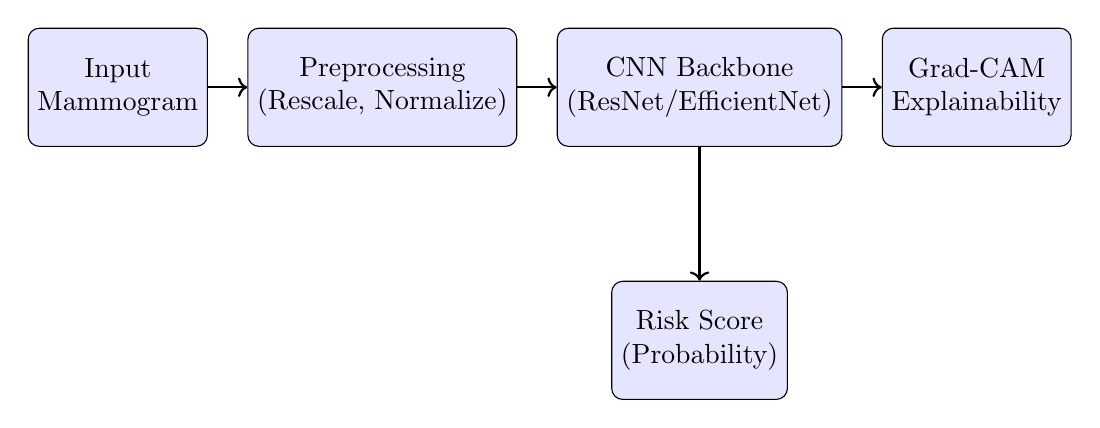
\begin{tikzpicture}[
        node distance=1cm and .5cm,
        box/.style={rectangle, draw=black, fill=blue!10, rounded corners, minimum width=1.5cm, minimum height=1.5cm, align=center},
        arrow/.style={->, thick}
        ]
        
        \node[box] (input) {Input\\Mammogram};
        \node[box, right=of input] (preprocess) {Preprocessing\\(Rescale, Normalize)};
        \node[box, right=of preprocess] (cnn) {CNN Backbone\\(ResNet/EfficientNet)};
        \node[box, right=of cnn] (gradcam) {Grad-CAM\\Explainability};
        \node[box, below=1.7cm of cnn] (output) {Risk Score\\(Probability)};
        
        \draw[arrow] (input) -- (preprocess);
        \draw[arrow] (preprocess) -- (cnn);
        \draw[arrow] (cnn) -- (gradcam);
        \draw[arrow] (cnn) -- (output);
    \end{tikzpicture}
    \caption{System architecture for explainable breast cancer risk prediction using convolutional neural networks (CNNs)~\cite{1} and Grad-CAM~\cite{5}.}
    \label{fig:system_architecture}
\end{figure}

Figure~\ref{fig:system_architecture} illustrates the overall pipeline. After preprocessing, images flow through a CNN for feature extraction~\cite{1}. One branch produces a risk score; the other passes through Grad-CAM~\cite{5} to generate attention heatmaps.

\paragraph{Design Considerations.}
Each module is deliberately kept modular and swappable. This enables future expansion, such as fine-tuning on Singaporean-specific data, incorporating metadata like patient history, or using multi-view mammography inputs~\cite{8}. This architectural flexibility ensures that the system can evolve as screening datasets, clinical requirements, and deployment contexts grow more complex.

In summary, this architecture reflects a balance between predictive strength and clinical usability—ensuring that both radiologists and patients benefit from a risk prediction system that is not only effective, but also transparent and adaptable.

\subsection{Dataset Used}

\paragraph{Primary Dataset – DDSM.}
The Digital Database for Screening Mammography (DDSM)~\cite{17} serves as the primary dataset. It comprises over 2,600 cases with four standard views per patient (cranio-caudal (CC) and mediolateral oblique (MLO) for each breast), along with verified pathology and ground-truth masks for abnormalities. This dataset provides a solid foundation for training and evaluating convolutional neural network (CNN)-based models due to its detailed annotation and diversity of tissue presentations. It contains both normal and cancerous cases, enabling the model to learn from contrastive examples.

\paragraph{Auxiliary Dataset – BreaKHis.}
The Breast Cancer Histopathological Image Classification (BreaKHis) dataset~\cite{18} is incorporated for auxiliary testing and domain adaptation experiments. Although histopathology data differ from mammograms, they offer complementary insights into cellular-level features and enable the project to explore cross-domain robustness.

\paragraph{Singapore-Specific Contextualization.}
Despite their value, both DDSM and BreaKHis originate from Western populations. To simulate Singaporean demographic conditions, stratified testing subsets will be constructed. Breast density and age distributions will be calibrated using data reported by the Singapore Breast Cancer Cohort~\cite{6} and the BreastScreen Singapore program~\cite{19}. Synthetic augmentation will mimic tissue characteristics more common among local women—such as denser fibroglandular tissue and smaller breast volume. This enables context-aware evaluation and reveals limitations in model generalizability.

\paragraph{Ethical Considerations.}
All datasets used are publicly available and de-identified, aligning with ethical guidelines for secondary use. In a future deployment scenario, local datasets such as those from National University Hospital (NUH) or Singapore General Hospital (SGH) could be integrated under appropriate ethics approval.

\vspace{1em}

\subsection{Feature Engineering}

Feature engineering is a critical bridge between raw mammographic data and effective CNN-based learning. As outlined in Figure~\ref{fig:end_to_end_pipeline}, this stage transforms high-resolution DICOM inputs into standardized, diverse, and clinically enriched representations suitable for training. The goal is to optimize generalization and sensitivity, particularly in dense breast tissue scenarios that are common among Singaporean women.

\begin{figure}[H]
    \centering
    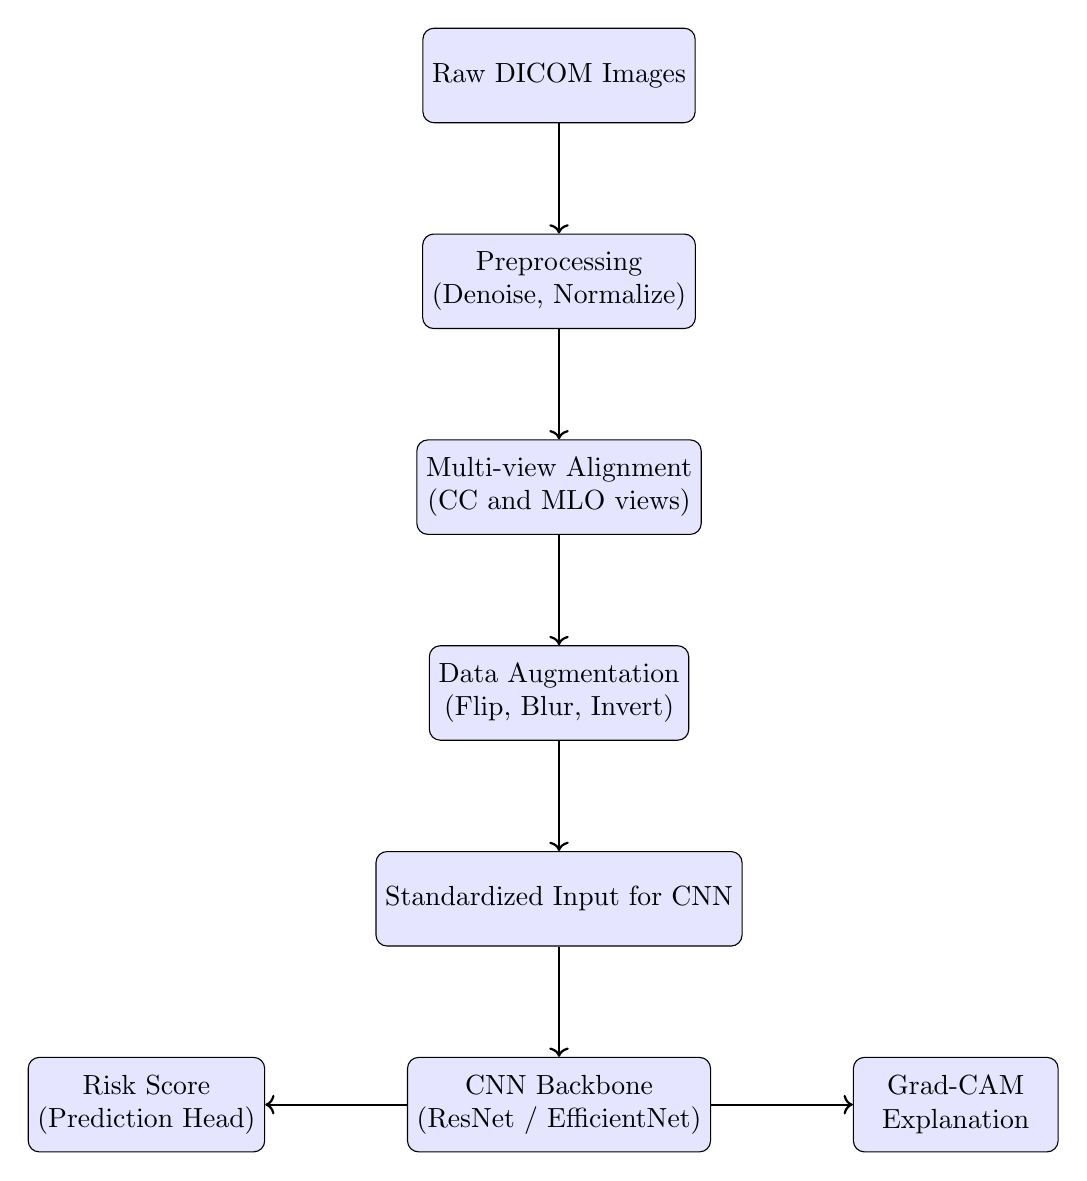
\begin{tikzpicture}[
        node distance=1.4cm and 0.8cm,
        box/.style={rectangle, draw=black, fill=blue!10, rounded corners, minimum width=2.6cm, minimum height=1.2cm, align=center},
        arrow/.style={->, thick}
        ]
        
        \node[box] (dicom) {Raw DICOM Images};
        \node[box, below=of dicom] (preprocess) {Preprocessing\\(Denoise, Normalize)};
        \node[box, below=of preprocess] (align) {Multi-view Alignment\\(CC and MLO views)};
        \node[box, below=of align] (augment) {Data Augmentation\\(Flip, Blur, Invert)};
        \node[box, below=of augment] (standard) {Standardized Input for CNN};
        \node[box, below=of standard] (cnn) {CNN Backbone\\(ResNet / EfficientNet)};
        \node[box, right=1.8cm of cnn] (gradcam) {Grad-CAM\\Explanation};
        \node[box, left=1.8cm of cnn] (score) {Risk Score\\(Prediction Head)};

        \draw[arrow] (dicom) -- (preprocess);
        \draw[arrow] (preprocess) -- (align);
        \draw[arrow] (align) -- (augment);
        \draw[arrow] (augment) -- (standard);
        \draw[arrow] (standard) -- (cnn);
        \draw[arrow] (cnn) -- (gradcam);
        \draw[arrow] (cnn) -- (score);
    \end{tikzpicture}
    \caption{End-to-end pipeline for breast cancer risk prediction, integrating preprocessing, multi-view feature alignment, CNN classification, and visual explainability.}
    \label{fig:end_to_end_pipeline}
\end{figure}

\paragraph{Preprocessing and Augmentation.}
The initial phase of feature engineering focuses on cleaning and enhancing the diagnostic quality of raw mammograms. This step is essential to ensure consistent model input and eliminate irrelevant imaging artifacts.

\begin{itemize}
    \item \textbf{Denoising:} Median filtering removes impulse noise (e.g., salt-and-pepper artifacts) while preserving fine structural detail—important for detecting subtle anomalies like microcalcifications.
    \item \textbf{Contrast enhancement:} CLAHE (contrast-limited adaptive histogram equalization)~\cite{14} enhances local contrast, improving visibility of faint lesions, especially in dense tissue environments.
    \item \textbf{Normalization:} Pixel values are rescaled to $[0,1]$ or z-normalized to ensure uniform dynamic range, enabling more stable model convergence.
\end{itemize}

After standardization, augmentation techniques are applied to increase data diversity and improve model robustness:

\begin{itemize}
    \item \textbf{Geometric:} Random flipping, cropping, and small-angle rotations ($\pm15^{\circ}$) simulate positioning variability during imaging.
    \item \textbf{Photometric:} Gaussian blurring and contrast jitter mimic scanner inconsistencies and imaging noise.
    \item \textbf{Semantic:} Intensity inversion introduces exposure variation and histogram shifts, improving cross-device generalization.
\end{itemize}

These transformations help prevent overfitting and prepare the model for deployment across heterogeneous clinical environments.

\paragraph{Multi-View Spatial Context.}
Breast screening typically involves multiple views: cranio-caudal (CC) and mediolateral oblique (MLO). Rather than treating each view independently, this project uses a multi-view strategy to leverage spatial correlations across angles. This is based on the approach by Geras et al.~\cite{8}, who showed that multi-view CNNs improve lesion localization and diagnostic accuracy.

\begin{figure}[H]
    \centering
    \includegraphics[width=0.95\textwidth]{images/GerasFig1.png}
    \caption{High-resolution mammogram processing via multi-view deep CNNs. Adapted from Geras et al.~\cite{8}.}
    \label{fig:geras}
\end{figure}

Both CC and MLO views are preprocessed and aligned to maintain anatomical consistency. This strategy enables the model to capture bilateral asymmetries, view-dependent lesion projections, and complementary diagnostic signals—critical for real-world screening reliability.

\paragraph{Domain-Specific Feature Emphasis.}
In addition to automated learning, domain knowledge is embedded to focus the model on clinically meaningful features:

\begin{itemize}
    \item \textbf{Asymmetry detection:} Breast difference maps highlight abnormal structural discrepancies between left and right sides.
    \item \textbf{Texture emphasis:} Gabor filters~\cite{20} are used to visualize texture patterns—such as spiculations—that are indicative of malignancy.
    \item \textbf{Density-informed stratification:} BI-RADS (Breast Imaging Reporting and Data System)~\cite{16} density levels are approximated via grayscale histograms and used to weight loss functions, placing more emphasis on dense cases that are diagnostically challenging.
\end{itemize}

These domain-guided strategies strengthen the model’s interpretability and diagnostic sensitivity. They also support the project’s goal of building a culturally adapted, clinically grounded AI system for breast cancer risk prediction.

\subsection{Algorithm Selection}
Chosen for its proven performance and balance of depth, ResNet-50 will serve as the initial benchmark. Its residual connections allow deeper gradient flow and faster convergence.

\paragraph{Alternative Models.}
Two models are benchmarked alongside ResNet:
\begin{itemize}
    \item \textbf{EfficientNet-B0:} Offers comparable accuracy with fewer parameters and reduced computation, ideal for edge deployment.
    \item \textbf{Custom Shallow CNN:} Inspired by Raghu et al.\ (2019), a smaller architecture trained from scratch will test the hypothesis that transfer learning from ImageNet is not always optimal in medical imaging.
\end{itemize}

\paragraph{Loss Function.}
Given the inherent class imbalance in breast cancer screening datasets—where malignant cases are relatively rare—choosing an appropriate loss function is crucial. The model is initially trained using Binary Cross-Entropy (BCE), a standard choice for binary classification tasks:

$$
\mathcal{L}_{\text{BCE}} = -\left[y \cdot \log(p) + (1 - y) \cdot \log(1 - p)\right]
$$

where $y \in \{0, 1\}$ is the ground truth label, and $p$ is the predicted probability of the positive (malignant) class.

However, BCE treats all samples equally, which may bias the model toward the dominant benign class. To mitigate this and better prioritize harder examples—particularly early-stage or subtle malignancies—a modified objective function, Focal Loss, is introduced:

$$
\mathcal{L}_{\text{focal}} = -\alpha_t(1 - p_t)^\gamma \log(p_t)
$$

Here, $p_t$ denotes the predicted probability for the ground truth class, $\alpha_t$ is a weighting factor to balance class contributions (e.g., higher for malignant), and $\gamma > 1$ is a focusing parameter. Setting $\gamma = 2$ reduces the loss contribution from easy examples and focuses learning on harder, misclassified cases. This is particularly valuable for enhancing sensitivity in dense breast tissue scenarios, where cancer detection is more challenging. The loss function thus directly supports the project's clinical objective of reducing false negatives in high-risk subgroups.

\paragraph{Optimization and Regularization.}
The Adam optimizer with a cyclical learning rate is used. Dropout layers are placed after the final dense layer to reduce overfitting. Early stopping with patience=10 is implemented.

\vspace{1em}

\subsection{Evaluation Metrics}

\paragraph{Quantitative Metrics.}
\begin{itemize}
    \item \textbf{AUC (Area Under the ROC Curve):} Primary metric to compare model discriminability, aligned with clinical risk score assessments.
    \item \textbf{Sensitivity \& Specificity:} Key indicators in screening settings. Sensitivity is emphasized to reduce false negatives.
    \item \textbf{F1-Score:} Provides a harmonic mean of precision and recall, especially relevant in imbalanced settings.
\end{itemize}

\paragraph{Explainability Evaluation.}
Grad-CAM heatmaps are overlaid on input mammograms and qualitatively scored by domain experts (when feasible) to assess alignment with tumor regions or diagnostic cues.

\begin{figure}[H]
    \centering
    \includegraphics[width=0.8\textwidth]{images/gradcam_sample.png}
    \caption{Grad-CAM visualizations showing model attention over mammograms. Red indicates regions of high diagnostic interest.}
\end{figure}

\paragraph{Qualitative Explainability Assessment.}
Beyond standard performance metrics, interpretability is essential in medical imaging. Kim et al.\ (2018) proposed the Data-driven Imaging Biomarker model (DIB-MG), which generates attention maps that highlight risk-relevant regions in mammograms. Their work supports my use of Grad-CAM as a means to validate model behavior against radiological intuition. As shown in Figure~\ref{fig:kim2018}, attention maps provide visual grounding for predictions, which is key to clinical trust and regulatory validation.

\begin{figure}[H]
    \centering
    \includegraphics[width=0.85\textwidth]{images/KimFig3.png}
    \caption{DIB-MG: Attention-based imaging biomarker model localizing high-risk regions. Adapted from Kim et al.\ (2018).}
    \label{fig:kim2018}
\end{figure}

\paragraph{Risk Stratification.}
Patients are ranked by predicted risk scores and divided into deciles. Metrics like:
\begin{itemize}
    \item \textbf{Cumulative incidence in top decile}
    \item \textbf{Hazard ratio (HR)}
    \item \textbf{Calibration curves}
\end{itemize}
are computed to evaluate clinical utility.

\paragraph{Cross-validation.}
A 5-fold stratified cross-validation is used during training. The final model is evaluated on a held-out test set to prevent data leakage and overfitting.

\vspace{1em}

\paragraph{Conclusion.}
This project adopts a structured, explainable deep learning architecture validated through standard and custom metrics. By leveraging Grad-CAM, dense tissue-aware training, and Singapore-specific context simulation, the design aligns both technically and clinically with the needs of under-screened populations in Southeast Asia.

\subsection{Work Plan and Project Timeline}

This project follows a structured timeline that spans from July to early September 2024. It is organized into four major phases:

\begin{enumerate}
    \item \textbf{Project Conceptualising (Weeks 1–5):} Includes idea formulation, early research, literature review, and preparation of briefing materials.
    \item \textbf{Project Planning and Design (Weeks 5–9):} Covers system design, prototyping, drafting of detailed work plans, and early-stage reporting.
    \item \textbf{Development and Testing (Weeks 10–18):} Encompasses data preprocessing, model development, training, validation, and initial evaluation.
    \item \textbf{Final Sprint (Weeks 18–25):} Focuses on final model evaluation, report writing, video presentation, and includes buffer time for contingency.
\end{enumerate}

Figure~\ref{fig:gantt} presents the visual Gantt chart outlining key tasks and deadlines, ensuring accountability across all milestones.

\begin{figure}[H]
    \centering
    \includegraphics[width=\textwidth]{images/GanttChart.png}
    \caption{Project Gantt chart showing planned activities from July to September 2024, divided into phases of research, development, evaluation, and reporting.}
    \label{fig:gantt}
\end{figure}

%-------------Feature Prototype Page-------------
\newpage
\section{Feature Prototype}
\subsection{Development Strategy}
\subsection{Evaluation}
\subsection{Improvements and Next Steps}

%-------------Appendices Page-------------
\newpage
\section{Appendices}

\subsection{Figures Referenced in Section 2.1: Limitations of Traditional Risk Models}

\begin{figure}[H]
    \centering
    \includegraphics[width=\textwidth]{images/lit1table2.png}
    \caption{Performance comparison between the Tyrer-Cuzick model and deep learning models across subgroups. Adapted from [1].}
    \label{fig:lit1table2}
\end{figure}

\subsection{Figures Referenced in Section 2.2: Role of Deep Learning in Breast Cancer Imaging}

\begin{figure}[H]
    \centering
    \includegraphics[width=0.9\textwidth]{images/hybrid_risk_by_density.png}
    \caption{Cancer incidence across density groups and hybrid risk scores. Adapted from [1].}
    \label{fig:hybrid_density}
\end{figure}

\begin{figure}[H]
    \centering
    \includegraphics[height=0.7\textheight]{images/lit1_roc_auc.png}
    \caption{ROC curves comparing Tyrer-Cuzick, image-only DL, and hybrid DL models. Adapted from [1].}
    \label{fig:lit1roc}
\end{figure}

\begin{figure}[H]
    \centering
    \includegraphics[width=0.85\textwidth]{images/ShenFig2.png}
    \caption{CNN-generated detection probabilities on mammograms. Adapted from [7].}
    \label{fig:shen2019}
\end{figure}

\subsection{Figure Referenced in Section 2.3: Explainability in Medical AI}

\begin{figure}[H]
    \centering
    \includegraphics[width=\textwidth]{images/gradcam_sample.png}
    \caption{Example of Grad-CAM heatmaps overlaid on mammograms, highlighting regions associated with high-risk predictions. Adapted from [5].}
    \label{fig:gradcam}
\end{figure}

\subsection{Figures Referenced in Section 2.4: Dataset Diversity and Generalization}

\begin{figure}[H]
    \centering
    \includegraphics[width=\textwidth]{images/lit2table7.png}
    \caption{Comparison of pretrained vs. randomly initialized CNNs in medical imaging tasks. Adapted from [2].}
    \label{fig:lit2table7}
\end{figure}

\subsection{Questionnaire / Lifestyle Simulation Input}
\subsection{Sample Transcriptions or Audio Prompts}

%-------------References Page-------------
\newpage
\section{References}
\begin{thebibliography}{99}

    \bibitem{1}
    A. Yala, C. Lehman, T. Schuster, T. Portnoi, and R. Barzilay. 2019. A Deep Learning Mammography-based Model for Improved Breast Cancer Risk Prediction. \textit{Radiology} 292, 1 (2019), 60–66. \url{https://pubs.rsna.org/doi/pdf/10.1148/radiol.2019182716}
    
    \bibitem{2}
    M. Raghu, C. Zhang, J. Kleinberg, and S. Bengio. 2019. Transfusion: Understanding Transfer Learning for Medical Imaging. In \textit{Proc. NeurIPS 2019}, 3342–3352. \url{https://proceedings.neurips.cc/paper/2019/file/eb1e78328c46506b46a4ac4a1e378b91-Paper.pdf}
    
    \bibitem{3}
    T. Ching, D. S. Himmelstein, B. K. Beaulieu-Jones, et al. 2018. Opportunities and obstacles for deep learning in biology and medicine. \textit{Nature Reviews Genetics} 19 (2018), 141–158. \url{https://royalsocietypublishing.org/doi/full/10.1098/rsif.2017.0387}
    
    \bibitem{4}
    V. Cheplygina, M. de Bruijne, and J. P. W. Pluim. 2019. Not-so-supervised: A survey of semi-supervised, multi-instance, and transfer learning in medical image analysis. \textit{Medical Image Analysis} 54 (2019), 280–296. \url{https://arxiv.org/pdf/1804.06353}
    
    \bibitem{5}
    R. R. Selvaraju, et al. 2017. Grad-CAM: Visual Explanations from Deep Networks via Gradient-based Localization. In \textit{Proc. ICCV}, 618–626. \url{https://openaccess.thecvf.com/content_ICCV_2017/papers/Selvaraju_Grad-CAM_Visual_Explanations_ICCV_2017_paper.pdf}
    
    \bibitem{6}
    W. Y. Chau, G. H. Lim, Y. L. Ng, et al. 2021. Breast density and breast cancer risk in Asian women: Evidence from the Singapore Breast Screening Programme. \textit{Cancer Epidemiology} 74 (2021), 101987. \url{https://pmc.ncbi.nlm.nih.gov/articles/PMC5160133/}
    
    \bibitem{7}
    L. Shen, L. R. Margolies, J. H. Rothstein, et al. 2019. Deep learning to improve breast cancer detection on screening mammography. \textit{Scientific Reports} 9, 1 (2019), 12495. \url{https://www.nature.com/articles/s41598-019-48995-4}
    
    \bibitem{8}
    K. J. Geras, S. Wolfson, Y. Shen, et al. 2017. High-resolution breast cancer screening with multi-view deep convolutional neural networks. \textit{arXiv preprint arXiv:1703.07047}. \url{https://arxiv.org/abs/1703.07047}
    
    \bibitem{9}
    H. J. Kim, E. Y. Ko, C. Kim, W. Han, and W. K. Moon. 2018. Applying Data-driven Imaging Biomarker in Mammography for Breast Cancer Screening: Preliminary Study. \textit{Scientific Reports} 8, 1 (2018), 12210. \url{https://www.ncbi.nlm.nih.gov/pmc/articles/PMC5807343/}
    
    \bibitem{10}
    National Registry of Diseases Office. 2021. \textit{Singapore Cancer Registry Annual Report 2021}. \url{https://www.nrdo.gov.sg/docs/librariesprovider3/publications-cancer/cancer2021.pdf}

    \bibitem{11}
    S. M. McKinney, M. Sieniek, V. Godbole, J. Godwin, N. Antropova, H. Ashrafian, et al. 2020. International evaluation of an AI system for breast cancer screening. \textit{Nature}, 577 (2020), 89–94. \url{https://www.nature.com/articles/s41586-019-1799-6}

    \bibitem{12}
    Zebra Medical Vision. 2021. Zebra’s AI1 Mammography Solutions. \url{https://www.zebra-med.com/}

    \bibitem{13}
    N. Salim, J. L. Andersson, A. Nordenskjöld, H. Svensson, K. Törnberg, and K. Zackrisson. 2024. Artificial intelligence for breast cancer screening in a real-world, population-based setting: cohort study of 58,000 mammograms. \textit{Nature Medicine}, (2024). \url{https://www.nature.com/articles/s41591-024-03061-0}

    \bibitem{14}
    J. Shen, L. Margolies, J. Rothstein, E. Fluder, R. McBride, and W. Sieh. 2019. Deep Learning to Improve Breast Cancer Detection on Screening Mammography. \textit{Scientific Reports} 9 (2019), 12495. \url{https://www.nature.com/articles/s41598-019-48995-4}

    \bibitem{14}
    K. Zuiderveld. 1994. Contrast Limited Adaptive Histogram Equalization. In P. S. Heckbert (Ed.), \textit{Graphics Gems IV}, 474–485. Academic Press. \url{https://doi.org/10.1016/B978-0-08-050755-2.50065-6}

    \bibitem{16}
    American College of Radiology. 2013. Breast Imaging Reporting and Data System (BI-RADS). \textit{ACR BI-RADS Atlas, Breast Imaging Reporting and Data System}. 5th Edition. American College of Radiology.

    \bibitem{17}
    K. He, X. Zhang, S. Ren, and J. Sun. 2016. Deep Residual Learning for Image Recognition. In \textit{Proc. CVPR}, 770–778. \url{https://doi.org/10.1109/CVPR.2016.90}

    \bibitem{18}
    M. Heath, K. Bowyer, D. Kopans, R. Moore, and W. P. Kegelmeyer. 2000. The Digital Database for Screening Mammography. In \textit{Proc. 5th International Workshop on Digital Mammography}, 212–218. \url{http://www.eng.usf.edu/cvprg/Mammography/Database.html}

    \bibitem{19}
    I. A. Spanhol, L. S. Oliveira, C. Petitjean, and L. Heutte. 2016. A dataset for breast cancer histopathological image classification. \textit{IEEE Transactions on Biomedical Engineering}, 63, 7 (2016), 1455–1462. \url{https://doi.org/10.1109/TBME.2015.2496264}

    \bibitem{20}
    J. Daugman. 1985. Uncertainty relation for resolution in space, spatial frequency, and orientation optimized by two-dimensional visual cortical filters. \textit{Journal of the Optical Society of America A}, 2, 7 (1985), 1160–1169. \url{https://doi.org/10.1364/JOSAA.2.001160}
    
    \end{thebibliography}
    
\end{document}